\subsection{Proposed workaround}

%
In the current approach, blocks are characterized using a fixed failure criteria on the output.
It results in a characterization table, describing the duration of the output disturbance from the width and amplitude of the input stimulus.
To remove and replace the failure criteria, the same exact approach is proposed.
Since the output duration is calculated with a table, then the output amplitude could be calculated using another table as well.

% New model description
The new model contains two 2D tables instead of one, and the new table associates an output amplitude to an input width and amplitude.
Fig. \ref{fig:principle-transfert-func-v2} summarizes the new model.
\textbf{Table A} is the amplitude table, to calculate the \textbf{amplitude} of the output disturbance.
\textbf{Table W} is the width table, to calculate the \textbf{duration} of the output disturbance.

\begin{figure}[!h]
  \centering
  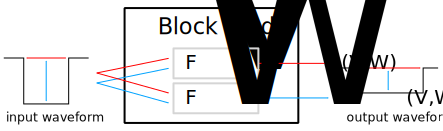
\includegraphics{src/4/figures/principle_transfert_function_v2.pdf}
  \caption{Improved modelling method}
  \label{fig:principle-transfert-func-v2}
\end{figure}

% What changes in the characterization
To extract both tables, the process is a bit different from the first methodology.
For each characterization simulation, the maximum output amplitude is recorded.
It is stored in table A.
The duration is measured on the output at 90\% of this maximum amplitude.
The validity of this threshold is discussed after in \ref{sec:limits-block-cz-final}.

% What does not change
The rest of the methodology remains identical.
In particular, model chaining is performed the same way since block models still accept and input width/disturbance and return an output width/disturbance.

% Summary of the process
%Fig. \ref{fig:full-method-v2} summarizes the entire characterization and chaining process for a 2-block setup.
%Each block is characterized, generating the two tables mentionned earlier.
%Then, using both tables, an input stress of 50V 100ns becomes a 12V 350ns disturbance after the first block, and a 3V 4000 ns after the second block.

%\begin{figure}[!h]
%  \centering
%  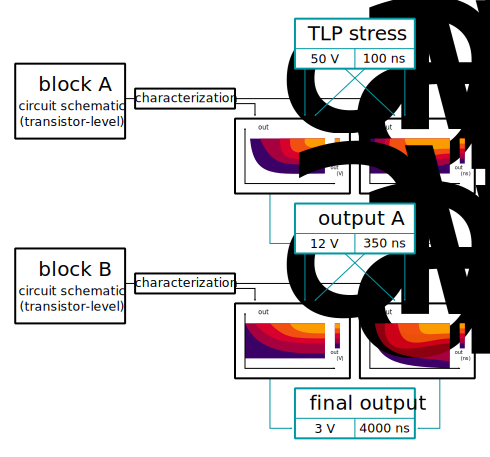
\includegraphics[width=0.7\textwidth]{src/4/figures/full_method_overview_v2.pdf}
%  \caption{Overview of improved bottom-up method - example with two blocks}
%  \label{fig:full-method-v2}
%\end{figure}

\subsubsection{Application of the improved method}

The new characterization method is applied to all three blocks of the regulation function.
The amplitude table of the pre-regulator is plotted in Fig. \ref{fig:pre_regu_amp} and the width table in Fig. \ref{fig:pre_regu_width}
Different patterns can be observed between both figures.
The amplitude gradient seems independent from the input width because it displays only horizontal lines, and depends only on the input amplitude.
The width matrix is a lot more complex with multiple different patterns.
Overall, large input amplitude and duration tend to result in long output disturbances.
Tables for the bandgap and pre-regulator are provided in Annex \ref{apx:block-cz}.

\begin{figure}[!h]
  \centering
  \includegraphics[width=\textwidth]{src/4/figures/vpre_cz_v2_amplitude.png}
  \caption{Pre-regulator V\textsubscript{clamp9} amplitude matrix}
  \label{fig:pre_regu_amp}
\end{figure}

\begin{figure}[!h]
  \centering
  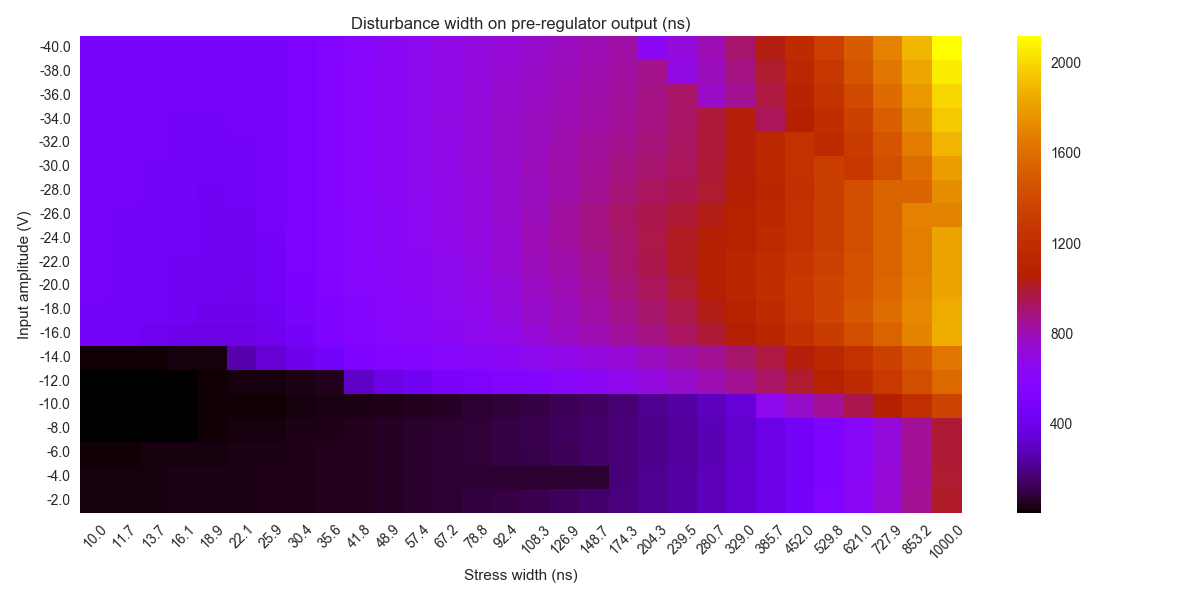
\includegraphics[width=\textwidth]{src/4/figures/vpre_cz_v2_width.png}
  \caption{Pre-regulator V\textsubscript{clamp9} width matrix}
  \label{fig:pre_regu_width}
\end{figure}


% TODO
% What is done for validation
To validate the changes, the chaining process...
The reference curve and reference test setups remain identical to the ones presented earlier (Fig. \ref{fig:reference_simu_circuit}).

% Result of the chaining process
The chaining process predicted that V\textsubscript{clamp9} will be down at -1.6V during 1800 ns.
In turn, V\textsubscript{1p0} was predicted at -1.25V during 3300 ns.
Finally, V\textsubscript{2p5} is predicted at 1.97V during 2700 ns.
Those values are employed for generating model waveforms.
They are compared to the reference simulation in Fig. \ref{fig:reference_simu_v2}.

% Curve analysis
The model matches correctly the simulation of V\textsubscript{clamp9}, both in terms of amplitude and width.
The width is slightly underestimated but overall the result is acceptable.
For V\textsubscript{1p0}, the width is extremely well reproduced, but the amplitude is about twice the reference value.
It seems that taking the minimum amplitude value during the characterization is not ideal.
This error should be investigated further to determine the actual root cause and provide a solution.
The last signal V\textsubscript{2p5} shows a quite good correlation despite the fact that it is a triangle-like waveform.
Overall, the modifications brought to the modelling method seemed to have a positive impact on the curve models.
A lot of room is left for improvements, in particular for reproducing the bandgap output signal.

\begin{figure}[!h]
  \centering
  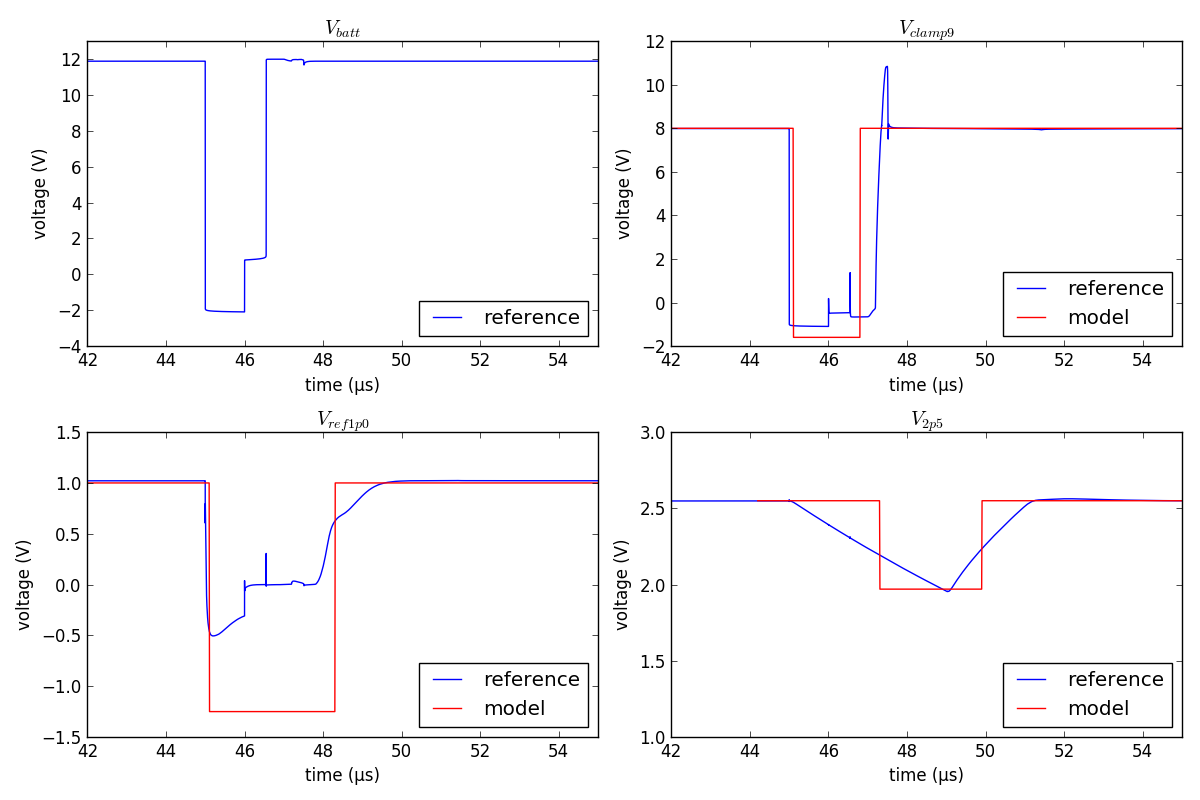
\includegraphics[width=\textwidth]{src/4/figures/total_simulation_30V_1u_V2.png}
  \caption{Reference simulation waveform - TLP stress -30V 1\textmugreek{}s }
  \label{fig:reference_simu_v2}
\end{figure}

% Conclusion, it works for this case
This section presented a potential improvement over the model chain method initially proposed.
This technique showed good results and seems promising for quickly estimating the robustness of a high-level integrated function.
The next section discusses further improvements for extracting width and amplitude during characterization.

\subsubsection{Potential improvements regarding parameters extraction}

% What is the challenge regarding the extraction of the models
In the simulations described earlier, a single width and maximum amplitude per waveform were extracted manually.
However, waveforms are never perfectly squared, and an width and amplitude cannot always be extracted easily.
The challenge is to find the right rule for simplifying them into a rectangular waveform, and extracting the two parameters.
This applies to the input waveform and the output waveform during the characterization of a block.

% First approach with a 90% amplitude
Initially, the rules were to set $V$ equal to the maximum value of the waveform (input or output), and $W$ the width of the pulse at 90\% of $V$.
The concept is illustrated in Fig. \ref{fig:impact-single-failure-criteria} with a few example curves.

\begin{figure}[!h]
  \centering
  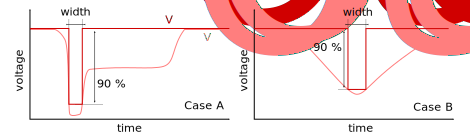
\includegraphics[width=0.98\textwidth]{src/4/figures/better_output_modelling.pdf}
  \caption{Improved output modelling method based on 90\% of maximum disturbance amplitude}
  \label{fig:impact-single-failure-criteria}
\end{figure}

% Problems with the 90% threshold
In case \textit{A}, the waveform can be simplified easily into a rectangular pulse.
However, this 90\% threshold does not work reliably with cases \textit{B} and \textit{C}.

% Explain case B
Case \textit{B} is often observed during the injection of an electrostatic discharge.
The \gls{esd} signal is superimposed on top of a slow signal variation.
In that case, the waveform exhibits a very short, high amplitude peak, followed by slower smaller-amplitude variation.
The width of the pulse is much shorter than the original curve, leading the model to be very inaccurate.

% Explain case C
Case \textit{C} is observed on nets with high capacitive coupling to ground.
Those signals are not directly disturbed by the \gls{esd}, but the block that drives them can go into reset.
In this situation, the nets slowly decreases then, once functionality resumes, the nets goes back to its nominal value.
With the 90\% threshold, a large area of the disturbed waveform is missing in the model, making it very inaccurate.

% What is the consequence
In both those cases, the 90\% threshold leads to underestimating the total disturbance width.
The modeled waveform has a much smaller duration and area than the original one.
Overall, it was observed that the model and original waveform areas should be close for the models to work.

% The relative threshold is not good enough, a smarter technique is required
Instead of focusing on the peak amplitude, a smarter method is required.
Ideally, it needs to extract a width and amplitude that would result in the same area than the original waveform, while looking as similar as possible.

%TODO
A feature detection method using amplitude distribution could be performed to identify key amplitudes in the waveforms.

\subsection{Limitations, conclusion and follow-up work}
\label{sec:limits-block-cz-final}

% Sum up what was done
In this section, principles were detailed for a block modeling method, targeting powered-on circuits exposed to disturbances.
It initially started off from the Wunsch and Bell method \cite{wunsch-bell}, which is based on a pass/fail failure criteria and targets hard-failure of electronic devices.
The method was improved to fit better the modeling of analog functions, symbolized by an input, and output and a transfer function.
The main modifications was to remove the use of a failure criteria, and record the severity of a disturbance through its duration and maximum amplitude.
For this purpose, waveforms observed on the inputs and outpus were simplified as rectangular shapes.
Then, lookup tables store the transient response of the characterized block against a wide range of input disturbance configurations.
On a single study-case, it was shown that this method works for predicting the failure of an output given an input stress.

% Limitations
Some limitations must be overcomed before this method can be applied to a larger scale.
So far, only very linear circuit topologies were considered.
A single input net and ouput net was studied per block.
It is one-to-one relation.
In reality, the relations are closer to many-to-one or many-to-many.
A single input will impact multiple outputs when disturbed.
Inputs do not have isolated impact, multiple inputs will affect the same group of outputs when they get stressed.

Also, more study cases are required to verify further the hypothesis under which ESD simulations at silicon-level can be performed using exclusively rectangular pulses, to disturb blocks in isolated testbenched.

%TODO?
%Section XX details a potential solution called electrical-simulations-as-a-service, acting as a drop-in replacement for tables models and black-box %models, that could solve this multiple-pin complexity issue.
